%------------------------------------------Packages used-------------------------------------------------
\documentclass[a4paper, 12pt, titlepage, oneside]{article}
\usepackage[utf8x]{inputenc}
\usepackage[english]{babel}
\usepackage[top=5em,left=6.5em, right=6.5em, bottom=5em]{geometry}
\usepackage{lipsum}
\usepackage{titling}
\usepackage{adjustbox}
\usepackage{tabularx}
\usepackage{amsmath,amssymb,amsfonts,amsthm}
\usepackage{graphicx}
\usepackage{microtype}
\usepackage{enumitem}
\usepackage[listings,theorems]{tcolorbox}
\usepackage{hyperref}
\usepackage{xcolor}
\usepackage{setspace}
\usepackage{fancyhdr}
\usepackage{wrapfig}

%--------------------------------------------------------------------------------------------------------
%%%Arduino Specific Packages and styles%%%
\usepackage{listings}
\lstset{
  language = Octave,
  backgroundcolor=\color{white},   
  basicstyle=\footnotesize\ttfamily,       
  breakatwhitespace=false,         
  breaklines=true,                 
  captionpos=b,                   
  commentstyle=\color{gray},    
  deletekeywords={...},           
  escapeinside={\%*}{*)},          
  extendedchars=true,              
  frame=single,
  framexleftmargin = 20pt,
  keepspaces=true,                 
  keywordstyle=\color{orange},       
  morekeywords={*,...},            
  numbers=left,                    
  numbersep=5pt,                   
  numberstyle=\footnotesize\color{gray}, 
  rulecolor=\color{black},         
  rulesepcolor=\color{blue},
  showspaces=false,                
  showstringspaces=false,          
  showtabs=false,                  
  stepnumber=1,                    
  stringstyle=\color{orange},    
  tabsize=2,                       
  title=\lstname,
  emphstyle=\bfseries\color{blue}%  style for emph={} 
} 
 %%%%%%%%%%%%%%%%%%%%%%%%%%%%%%%%%%%%%%%%%%%%%%%%%%%%%%%%%%%%%%%%%%%%%%%%%%%%%%%% 
%%% ~ Arduino Language - Arduino IDE Colors ~                                  %%%
%%%                                                                            %%%
%%% Kyle Rocha-Brownell | 10/2/2017 | No Licence                               %%%
%%% -------------------------------------------------------------------------- %%%
%%%                                                                            %%%
%%% Place this file in your working directory (next to the latex file you're   %%%
%%% working on).  To add it to your project, place:                            %%%
%%%     %%%%%%%%%%%%%%%%%%%%%%%%%%%%%%%%%%%%%%%%%%%%%%%%%%%%%%%%%%%%%%%%%%%%%%%%%%%%%%%% 
%%% ~ Arduino Language - Arduino IDE Colors ~                                  %%%
%%%                                                                            %%%
%%% Kyle Rocha-Brownell | 10/2/2017 | No Licence                               %%%
%%% -------------------------------------------------------------------------- %%%
%%%                                                                            %%%
%%% Place this file in your working directory (next to the latex file you're   %%%
%%% working on).  To add it to your project, place:                            %%%
%%%     %%%%%%%%%%%%%%%%%%%%%%%%%%%%%%%%%%%%%%%%%%%%%%%%%%%%%%%%%%%%%%%%%%%%%%%%%%%%%%%% 
%%% ~ Arduino Language - Arduino IDE Colors ~                                  %%%
%%%                                                                            %%%
%%% Kyle Rocha-Brownell | 10/2/2017 | No Licence                               %%%
%%% -------------------------------------------------------------------------- %%%
%%%                                                                            %%%
%%% Place this file in your working directory (next to the latex file you're   %%%
%%% working on).  To add it to your project, place:                            %%%
%%%    \input{arduinoLanguage.tex}                                             %%%
%%% somewhere before \begin{document} in your latex file.                      %%%
%%%                                                                            %%%
%%% In your document, place your arduino code between:                         %%%
%%%   \begin{lstlisting}[language=Arduino]                                     %%%
%%% and:                                                                       %%%
%%%   \end{lstlisting}                                                         %%%
%%%                                                                            %%%
%%% Or create your own style to add non-built-in functions and variables.      %%%
%%%                                                                            %%%
 %%%%%%%%%%%%%%%%%%%%%%%%%%%%%%%%%%%%%%%%%%%%%%%%%%%%%%%%%%%%%%%%%%%%%%%%%%%%%%%% 

\usepackage{color}
\usepackage{listings}    
\usepackage{courier}

%%% Define Custom IDE Colors %%%
\definecolor{arduinoGreen}    {rgb} {0.17, 0.43, 0.01}
\definecolor{arduinoGrey}     {rgb} {0.47, 0.47, 0.33}
\definecolor{arduinoOrange}   {rgb} {0.8 , 0.4 , 0   }
\definecolor{arduinoBlue}     {rgb} {0.01, 0.61, 0.98}
\definecolor{arduinoDarkBlue} {rgb} {0.0 , 0.2 , 0.5 }

%%% Define Arduino Language %%%
\lstdefinelanguage{Arduino}{
  language=C++, % begin with default C++ settings 
%
%
  %%% Keyword Color Group 1 %%%  (called KEYWORD3 by arduino)
  keywordstyle=\color{arduinoGreen},   
  deletekeywords={  % remove all arduino keywords that might be in c++
                break, case, override, final, continue, default, do, else, for, 
                if, return, goto, switch, throw, try, while, setup, loop, export, 
                not, or, and, xor, include, define, elif, else, error, if, ifdef, 
                ifndef, pragma, warning,
                HIGH, LOW, INPUT, INPUT_PULLUP, OUTPUT, DEC, BIN, HEX, OCT, PI, 
                HALF_PI, TWO_PI, LSBFIRST, MSBFIRST, CHANGE, FALLING, RISING, 
                DEFAULT, EXTERNAL, INTERNAL, INTERNAL1V1, INTERNAL2V56, LED_BUILTIN, 
                LED_BUILTIN_RX, LED_BUILTIN_TX, DIGITAL_MESSAGE, FIRMATA_STRING, 
                ANALOG_MESSAGE, REPORT_DIGITAL, REPORT_ANALOG, SET_PIN_MODE, 
                SYSTEM_RESET, SYSEX_START, auto, int8_t, int16_t, int32_t, int64_t, 
                uint8_t, uint16_t, uint32_t, uint64_t, char16_t, char32_t, operator, 
                enum, delete, bool, boolean, byte, char, const, false, float, double, 
                null, NULL, int, long, new, private, protected, public, short, 
                signed, static, volatile, String, void, true, unsigned, word, array, 
                sizeof, dynamic_cast, typedef, const_cast, struct, static_cast, union, 
                friend, extern, class, reinterpret_cast, register, explicit, inline, 
                _Bool, complex, _Complex, _Imaginary, atomic_bool, atomic_char, 
                atomic_schar, atomic_uchar, atomic_short, atomic_ushort, atomic_int, 
                atomic_uint, atomic_long, atomic_ulong, atomic_llong, atomic_ullong, 
                virtual, PROGMEM,
                Serial, Serial1, Serial2, Serial3, SerialUSB, Keyboard, Mouse,
                abs, acos, asin, atan, atan2, ceil, constrain, cos, degrees, exp, 
                floor, log, map, max, min, radians, random, randomSeed, round, sin, 
                sq, sqrt, tan, pow, bitRead, bitWrite, bitSet, bitClear, bit, 
                highByte, lowByte, analogReference, analogRead, 
                analogReadResolution, analogWrite, analogWriteResolution, 
                attachInterrupt, detachInterrupt, digitalPinToInterrupt, delay, 
                delayMicroseconds, digitalWrite, digitalRead, interrupts, millis, 
                micros, noInterrupts, noTone, pinMode, pulseIn, pulseInLong, shiftIn, 
                shiftOut, tone, yield, Stream, begin, end, peek, read, print, 
                println, available, availableForWrite, flush, setTimeout, find, 
                findUntil, parseInt, parseFloat, readBytes, readBytesUntil, readString, 
                readStringUntil, trim, toUpperCase, toLowerCase, charAt, compareTo, 
                concat, endsWith, startsWith, equals, equalsIgnoreCase, getBytes, 
                indexOf, lastIndexOf, length, replace, setCharAt, substring, 
                toCharArray, toInt, press, release, releaseAll, accept, click, move, 
                isPressed, isAlphaNumeric, isAlpha, isAscii, isWhitespace, isControl, 
                isDigit, isGraph, isLowerCase, isPrintable, isPunct, isSpace, 
                isUpperCase, isHexadecimalDigit, 
                }, 
  morekeywords={   % add arduino structures to group 1
                break, case, override, final, continue, default, do, else, for, 
                if, return, goto, switch, throw, try, while, setup, loop, export, 
                not, or, and, xor, include, define, elif, else, error, if, ifdef, 
                ifndef, pragma, warning,
                }, 
% 
%
  %%% Keyword Color Group 2 %%%  (called LITERAL1 by arduino)
  keywordstyle=[2]\color{arduinoBlue},   
  keywords=[2]{   % add variables and dataTypes as 2nd group  
                HIGH, LOW, INPUT, INPUT_PULLUP, OUTPUT, DEC, BIN, HEX, OCT, PI, 
                HALF_PI, TWO_PI, LSBFIRST, MSBFIRST, CHANGE, FALLING, RISING, 
                DEFAULT, EXTERNAL, INTERNAL, INTERNAL1V1, INTERNAL2V56, LED_BUILTIN, 
                LED_BUILTIN_RX, LED_BUILTIN_TX, DIGITAL_MESSAGE, FIRMATA_STRING, 
                ANALOG_MESSAGE, REPORT_DIGITAL, REPORT_ANALOG, SET_PIN_MODE, 
                SYSTEM_RESET, SYSEX_START, auto, int8_t, int16_t, int32_t, int64_t, 
                uint8_t, uint16_t, uint32_t, uint64_t, char16_t, char32_t, operator, 
                enum, delete, bool, boolean, byte, char, const, false, float, double, 
                null, NULL, int, long, new, private, protected, public, short, 
                signed, static, volatile, String, void, true, unsigned, word, array, 
                sizeof, dynamic_cast, typedef, const_cast, struct, static_cast, union, 
                friend, extern, class, reinterpret_cast, register, explicit, inline, 
                _Bool, complex, _Complex, _Imaginary, atomic_bool, atomic_char, 
                atomic_schar, atomic_uchar, atomic_short, atomic_ushort, atomic_int, 
                atomic_uint, atomic_long, atomic_ulong, atomic_llong, atomic_ullong, 
                virtual, PROGMEM,
                },  
% 
%
  %%% Keyword Color Group 3 %%%  (called KEYWORD1 by arduino)
  keywordstyle=[3]\bfseries\color{arduinoOrange},
  keywords=[3]{  % add built-in functions as a 3rd group
                Serial, Serial1, Serial2, Serial3, SerialUSB, Keyboard, Mouse,
                },      
%
%
  %%% Keyword Color Group 4 %%%  (called KEYWORD2 by arduino)
  keywordstyle=[4]\color{arduinoOrange},
  keywords=[4]{  % add more built-in functions as a 4th group
                abs, acos, asin, atan, atan2, ceil, constrain, cos, degrees, exp, 
                floor, log, map, max, min, radians, random, randomSeed, round, sin, 
                sq, sqrt, tan, pow, bitRead, bitWrite, bitSet, bitClear, bit, 
                highByte, lowByte, analogReference, analogRead, 
                analogReadResolution, analogWrite, analogWriteResolution, 
                attachInterrupt, detachInterrupt, digitalPinToInterrupt, delay, 
                delayMicroseconds, digitalWrite, digitalRead, interrupts, millis, 
                micros, noInterrupts, noTone, pinMode, pulseIn, pulseInLong, shiftIn, 
                shiftOut, tone, yield, Stream, begin, end, peek, read, print, 
                println, available, availableForWrite, flush, setTimeout, find, 
                findUntil, parseInt, parseFloat, readBytes, readBytesUntil, readString, 
                readStringUntil, trim, toUpperCase, toLowerCase, charAt, compareTo, 
                concat, endsWith, startsWith, equals, equalsIgnoreCase, getBytes, 
                indexOf, lastIndexOf, length, replace, setCharAt, substring, 
                toCharArray, toInt, press, release, releaseAll, accept, click, move, 
                isPressed, isAlphaNumeric, isAlpha, isAscii, isWhitespace, isControl, 
                isDigit, isGraph, isLowerCase, isPrintable, isPunct, isSpace, 
                isUpperCase, isHexadecimalDigit, 
                },      
%
%
  %%% Set Other Colors %%%
  stringstyle=\color{arduinoDarkBlue},    
  commentstyle=\color{arduinoGrey},    
%          
%   
  %%%% Line Numbering %%%%
  numbers=left,                    
  numbersep=5pt,                   
  numberstyle=\color{arduinoGrey},    
  %stepnumber=2,                      % show every 2 line numbers
%
%
  %%%% Code Box Style %%%%
  breaklines=true,                    % wordwrapping
  tabsize=2,         
  basicstyle=\ttfamily  
}                                             %%%
%%% somewhere before \begin{document} in your latex file.                      %%%
%%%                                                                            %%%
%%% In your document, place your arduino code between:                         %%%
%%%   \begin{lstlisting}[language=Arduino]                                     %%%
%%% and:                                                                       %%%
%%%   \end{lstlisting}                                                         %%%
%%%                                                                            %%%
%%% Or create your own style to add non-built-in functions and variables.      %%%
%%%                                                                            %%%
 %%%%%%%%%%%%%%%%%%%%%%%%%%%%%%%%%%%%%%%%%%%%%%%%%%%%%%%%%%%%%%%%%%%%%%%%%%%%%%%% 

\usepackage{color}
\usepackage{listings}    
\usepackage{courier}

%%% Define Custom IDE Colors %%%
\definecolor{arduinoGreen}    {rgb} {0.17, 0.43, 0.01}
\definecolor{arduinoGrey}     {rgb} {0.47, 0.47, 0.33}
\definecolor{arduinoOrange}   {rgb} {0.8 , 0.4 , 0   }
\definecolor{arduinoBlue}     {rgb} {0.01, 0.61, 0.98}
\definecolor{arduinoDarkBlue} {rgb} {0.0 , 0.2 , 0.5 }

%%% Define Arduino Language %%%
\lstdefinelanguage{Arduino}{
  language=C++, % begin with default C++ settings 
%
%
  %%% Keyword Color Group 1 %%%  (called KEYWORD3 by arduino)
  keywordstyle=\color{arduinoGreen},   
  deletekeywords={  % remove all arduino keywords that might be in c++
                break, case, override, final, continue, default, do, else, for, 
                if, return, goto, switch, throw, try, while, setup, loop, export, 
                not, or, and, xor, include, define, elif, else, error, if, ifdef, 
                ifndef, pragma, warning,
                HIGH, LOW, INPUT, INPUT_PULLUP, OUTPUT, DEC, BIN, HEX, OCT, PI, 
                HALF_PI, TWO_PI, LSBFIRST, MSBFIRST, CHANGE, FALLING, RISING, 
                DEFAULT, EXTERNAL, INTERNAL, INTERNAL1V1, INTERNAL2V56, LED_BUILTIN, 
                LED_BUILTIN_RX, LED_BUILTIN_TX, DIGITAL_MESSAGE, FIRMATA_STRING, 
                ANALOG_MESSAGE, REPORT_DIGITAL, REPORT_ANALOG, SET_PIN_MODE, 
                SYSTEM_RESET, SYSEX_START, auto, int8_t, int16_t, int32_t, int64_t, 
                uint8_t, uint16_t, uint32_t, uint64_t, char16_t, char32_t, operator, 
                enum, delete, bool, boolean, byte, char, const, false, float, double, 
                null, NULL, int, long, new, private, protected, public, short, 
                signed, static, volatile, String, void, true, unsigned, word, array, 
                sizeof, dynamic_cast, typedef, const_cast, struct, static_cast, union, 
                friend, extern, class, reinterpret_cast, register, explicit, inline, 
                _Bool, complex, _Complex, _Imaginary, atomic_bool, atomic_char, 
                atomic_schar, atomic_uchar, atomic_short, atomic_ushort, atomic_int, 
                atomic_uint, atomic_long, atomic_ulong, atomic_llong, atomic_ullong, 
                virtual, PROGMEM,
                Serial, Serial1, Serial2, Serial3, SerialUSB, Keyboard, Mouse,
                abs, acos, asin, atan, atan2, ceil, constrain, cos, degrees, exp, 
                floor, log, map, max, min, radians, random, randomSeed, round, sin, 
                sq, sqrt, tan, pow, bitRead, bitWrite, bitSet, bitClear, bit, 
                highByte, lowByte, analogReference, analogRead, 
                analogReadResolution, analogWrite, analogWriteResolution, 
                attachInterrupt, detachInterrupt, digitalPinToInterrupt, delay, 
                delayMicroseconds, digitalWrite, digitalRead, interrupts, millis, 
                micros, noInterrupts, noTone, pinMode, pulseIn, pulseInLong, shiftIn, 
                shiftOut, tone, yield, Stream, begin, end, peek, read, print, 
                println, available, availableForWrite, flush, setTimeout, find, 
                findUntil, parseInt, parseFloat, readBytes, readBytesUntil, readString, 
                readStringUntil, trim, toUpperCase, toLowerCase, charAt, compareTo, 
                concat, endsWith, startsWith, equals, equalsIgnoreCase, getBytes, 
                indexOf, lastIndexOf, length, replace, setCharAt, substring, 
                toCharArray, toInt, press, release, releaseAll, accept, click, move, 
                isPressed, isAlphaNumeric, isAlpha, isAscii, isWhitespace, isControl, 
                isDigit, isGraph, isLowerCase, isPrintable, isPunct, isSpace, 
                isUpperCase, isHexadecimalDigit, 
                }, 
  morekeywords={   % add arduino structures to group 1
                break, case, override, final, continue, default, do, else, for, 
                if, return, goto, switch, throw, try, while, setup, loop, export, 
                not, or, and, xor, include, define, elif, else, error, if, ifdef, 
                ifndef, pragma, warning,
                }, 
% 
%
  %%% Keyword Color Group 2 %%%  (called LITERAL1 by arduino)
  keywordstyle=[2]\color{arduinoBlue},   
  keywords=[2]{   % add variables and dataTypes as 2nd group  
                HIGH, LOW, INPUT, INPUT_PULLUP, OUTPUT, DEC, BIN, HEX, OCT, PI, 
                HALF_PI, TWO_PI, LSBFIRST, MSBFIRST, CHANGE, FALLING, RISING, 
                DEFAULT, EXTERNAL, INTERNAL, INTERNAL1V1, INTERNAL2V56, LED_BUILTIN, 
                LED_BUILTIN_RX, LED_BUILTIN_TX, DIGITAL_MESSAGE, FIRMATA_STRING, 
                ANALOG_MESSAGE, REPORT_DIGITAL, REPORT_ANALOG, SET_PIN_MODE, 
                SYSTEM_RESET, SYSEX_START, auto, int8_t, int16_t, int32_t, int64_t, 
                uint8_t, uint16_t, uint32_t, uint64_t, char16_t, char32_t, operator, 
                enum, delete, bool, boolean, byte, char, const, false, float, double, 
                null, NULL, int, long, new, private, protected, public, short, 
                signed, static, volatile, String, void, true, unsigned, word, array, 
                sizeof, dynamic_cast, typedef, const_cast, struct, static_cast, union, 
                friend, extern, class, reinterpret_cast, register, explicit, inline, 
                _Bool, complex, _Complex, _Imaginary, atomic_bool, atomic_char, 
                atomic_schar, atomic_uchar, atomic_short, atomic_ushort, atomic_int, 
                atomic_uint, atomic_long, atomic_ulong, atomic_llong, atomic_ullong, 
                virtual, PROGMEM,
                },  
% 
%
  %%% Keyword Color Group 3 %%%  (called KEYWORD1 by arduino)
  keywordstyle=[3]\bfseries\color{arduinoOrange},
  keywords=[3]{  % add built-in functions as a 3rd group
                Serial, Serial1, Serial2, Serial3, SerialUSB, Keyboard, Mouse,
                },      
%
%
  %%% Keyword Color Group 4 %%%  (called KEYWORD2 by arduino)
  keywordstyle=[4]\color{arduinoOrange},
  keywords=[4]{  % add more built-in functions as a 4th group
                abs, acos, asin, atan, atan2, ceil, constrain, cos, degrees, exp, 
                floor, log, map, max, min, radians, random, randomSeed, round, sin, 
                sq, sqrt, tan, pow, bitRead, bitWrite, bitSet, bitClear, bit, 
                highByte, lowByte, analogReference, analogRead, 
                analogReadResolution, analogWrite, analogWriteResolution, 
                attachInterrupt, detachInterrupt, digitalPinToInterrupt, delay, 
                delayMicroseconds, digitalWrite, digitalRead, interrupts, millis, 
                micros, noInterrupts, noTone, pinMode, pulseIn, pulseInLong, shiftIn, 
                shiftOut, tone, yield, Stream, begin, end, peek, read, print, 
                println, available, availableForWrite, flush, setTimeout, find, 
                findUntil, parseInt, parseFloat, readBytes, readBytesUntil, readString, 
                readStringUntil, trim, toUpperCase, toLowerCase, charAt, compareTo, 
                concat, endsWith, startsWith, equals, equalsIgnoreCase, getBytes, 
                indexOf, lastIndexOf, length, replace, setCharAt, substring, 
                toCharArray, toInt, press, release, releaseAll, accept, click, move, 
                isPressed, isAlphaNumeric, isAlpha, isAscii, isWhitespace, isControl, 
                isDigit, isGraph, isLowerCase, isPrintable, isPunct, isSpace, 
                isUpperCase, isHexadecimalDigit, 
                },      
%
%
  %%% Set Other Colors %%%
  stringstyle=\color{arduinoDarkBlue},    
  commentstyle=\color{arduinoGrey},    
%          
%   
  %%%% Line Numbering %%%%
  numbers=left,                    
  numbersep=5pt,                   
  numberstyle=\color{arduinoGrey},    
  %stepnumber=2,                      % show every 2 line numbers
%
%
  %%%% Code Box Style %%%%
  breaklines=true,                    % wordwrapping
  tabsize=2,         
  basicstyle=\ttfamily  
}                                             %%%
%%% somewhere before \begin{document} in your latex file.                      %%%
%%%                                                                            %%%
%%% In your document, place your arduino code between:                         %%%
%%%   \begin{lstlisting}[language=Arduino]                                     %%%
%%% and:                                                                       %%%
%%%   \end{lstlisting}                                                         %%%
%%%                                                                            %%%
%%% Or create your own style to add non-built-in functions and variables.      %%%
%%%                                                                            %%%
 %%%%%%%%%%%%%%%%%%%%%%%%%%%%%%%%%%%%%%%%%%%%%%%%%%%%%%%%%%%%%%%%%%%%%%%%%%%%%%%% 

\usepackage{color}
\usepackage{listings}    
\usepackage{courier}

%%% Define Custom IDE Colors %%%
\definecolor{arduinoGreen}    {rgb} {0.17, 0.43, 0.01}
\definecolor{arduinoGrey}     {rgb} {0.47, 0.47, 0.33}
\definecolor{arduinoOrange}   {rgb} {0.8 , 0.4 , 0   }
\definecolor{arduinoBlue}     {rgb} {0.01, 0.61, 0.98}
\definecolor{arduinoDarkBlue} {rgb} {0.0 , 0.2 , 0.5 }

%%% Define Arduino Language %%%
\lstdefinelanguage{Arduino}{
  language=C++, % begin with default C++ settings 
%
%
  %%% Keyword Color Group 1 %%%  (called KEYWORD3 by arduino)
  keywordstyle=\color{arduinoGreen},   
  deletekeywords={  % remove all arduino keywords that might be in c++
                break, case, override, final, continue, default, do, else, for, 
                if, return, goto, switch, throw, try, while, setup, loop, export, 
                not, or, and, xor, include, define, elif, else, error, if, ifdef, 
                ifndef, pragma, warning,
                HIGH, LOW, INPUT, INPUT_PULLUP, OUTPUT, DEC, BIN, HEX, OCT, PI, 
                HALF_PI, TWO_PI, LSBFIRST, MSBFIRST, CHANGE, FALLING, RISING, 
                DEFAULT, EXTERNAL, INTERNAL, INTERNAL1V1, INTERNAL2V56, LED_BUILTIN, 
                LED_BUILTIN_RX, LED_BUILTIN_TX, DIGITAL_MESSAGE, FIRMATA_STRING, 
                ANALOG_MESSAGE, REPORT_DIGITAL, REPORT_ANALOG, SET_PIN_MODE, 
                SYSTEM_RESET, SYSEX_START, auto, int8_t, int16_t, int32_t, int64_t, 
                uint8_t, uint16_t, uint32_t, uint64_t, char16_t, char32_t, operator, 
                enum, delete, bool, boolean, byte, char, const, false, float, double, 
                null, NULL, int, long, new, private, protected, public, short, 
                signed, static, volatile, String, void, true, unsigned, word, array, 
                sizeof, dynamic_cast, typedef, const_cast, struct, static_cast, union, 
                friend, extern, class, reinterpret_cast, register, explicit, inline, 
                _Bool, complex, _Complex, _Imaginary, atomic_bool, atomic_char, 
                atomic_schar, atomic_uchar, atomic_short, atomic_ushort, atomic_int, 
                atomic_uint, atomic_long, atomic_ulong, atomic_llong, atomic_ullong, 
                virtual, PROGMEM,
                Serial, Serial1, Serial2, Serial3, SerialUSB, Keyboard, Mouse,
                abs, acos, asin, atan, atan2, ceil, constrain, cos, degrees, exp, 
                floor, log, map, max, min, radians, random, randomSeed, round, sin, 
                sq, sqrt, tan, pow, bitRead, bitWrite, bitSet, bitClear, bit, 
                highByte, lowByte, analogReference, analogRead, 
                analogReadResolution, analogWrite, analogWriteResolution, 
                attachInterrupt, detachInterrupt, digitalPinToInterrupt, delay, 
                delayMicroseconds, digitalWrite, digitalRead, interrupts, millis, 
                micros, noInterrupts, noTone, pinMode, pulseIn, pulseInLong, shiftIn, 
                shiftOut, tone, yield, Stream, begin, end, peek, read, print, 
                println, available, availableForWrite, flush, setTimeout, find, 
                findUntil, parseInt, parseFloat, readBytes, readBytesUntil, readString, 
                readStringUntil, trim, toUpperCase, toLowerCase, charAt, compareTo, 
                concat, endsWith, startsWith, equals, equalsIgnoreCase, getBytes, 
                indexOf, lastIndexOf, length, replace, setCharAt, substring, 
                toCharArray, toInt, press, release, releaseAll, accept, click, move, 
                isPressed, isAlphaNumeric, isAlpha, isAscii, isWhitespace, isControl, 
                isDigit, isGraph, isLowerCase, isPrintable, isPunct, isSpace, 
                isUpperCase, isHexadecimalDigit, 
                }, 
  morekeywords={   % add arduino structures to group 1
                break, case, override, final, continue, default, do, else, for, 
                if, return, goto, switch, throw, try, while, setup, loop, export, 
                not, or, and, xor, include, define, elif, else, error, if, ifdef, 
                ifndef, pragma, warning,
                }, 
% 
%
  %%% Keyword Color Group 2 %%%  (called LITERAL1 by arduino)
  keywordstyle=[2]\color{arduinoBlue},   
  keywords=[2]{   % add variables and dataTypes as 2nd group  
                HIGH, LOW, INPUT, INPUT_PULLUP, OUTPUT, DEC, BIN, HEX, OCT, PI, 
                HALF_PI, TWO_PI, LSBFIRST, MSBFIRST, CHANGE, FALLING, RISING, 
                DEFAULT, EXTERNAL, INTERNAL, INTERNAL1V1, INTERNAL2V56, LED_BUILTIN, 
                LED_BUILTIN_RX, LED_BUILTIN_TX, DIGITAL_MESSAGE, FIRMATA_STRING, 
                ANALOG_MESSAGE, REPORT_DIGITAL, REPORT_ANALOG, SET_PIN_MODE, 
                SYSTEM_RESET, SYSEX_START, auto, int8_t, int16_t, int32_t, int64_t, 
                uint8_t, uint16_t, uint32_t, uint64_t, char16_t, char32_t, operator, 
                enum, delete, bool, boolean, byte, char, const, false, float, double, 
                null, NULL, int, long, new, private, protected, public, short, 
                signed, static, volatile, String, void, true, unsigned, word, array, 
                sizeof, dynamic_cast, typedef, const_cast, struct, static_cast, union, 
                friend, extern, class, reinterpret_cast, register, explicit, inline, 
                _Bool, complex, _Complex, _Imaginary, atomic_bool, atomic_char, 
                atomic_schar, atomic_uchar, atomic_short, atomic_ushort, atomic_int, 
                atomic_uint, atomic_long, atomic_ulong, atomic_llong, atomic_ullong, 
                virtual, PROGMEM,
                },  
% 
%
  %%% Keyword Color Group 3 %%%  (called KEYWORD1 by arduino)
  keywordstyle=[3]\bfseries\color{arduinoOrange},
  keywords=[3]{  % add built-in functions as a 3rd group
                Serial, Serial1, Serial2, Serial3, SerialUSB, Keyboard, Mouse,
                },      
%
%
  %%% Keyword Color Group 4 %%%  (called KEYWORD2 by arduino)
  keywordstyle=[4]\color{arduinoOrange},
  keywords=[4]{  % add more built-in functions as a 4th group
                abs, acos, asin, atan, atan2, ceil, constrain, cos, degrees, exp, 
                floor, log, map, max, min, radians, random, randomSeed, round, sin, 
                sq, sqrt, tan, pow, bitRead, bitWrite, bitSet, bitClear, bit, 
                highByte, lowByte, analogReference, analogRead, 
                analogReadResolution, analogWrite, analogWriteResolution, 
                attachInterrupt, detachInterrupt, digitalPinToInterrupt, delay, 
                delayMicroseconds, digitalWrite, digitalRead, interrupts, millis, 
                micros, noInterrupts, noTone, pinMode, pulseIn, pulseInLong, shiftIn, 
                shiftOut, tone, yield, Stream, begin, end, peek, read, print, 
                println, available, availableForWrite, flush, setTimeout, find, 
                findUntil, parseInt, parseFloat, readBytes, readBytesUntil, readString, 
                readStringUntil, trim, toUpperCase, toLowerCase, charAt, compareTo, 
                concat, endsWith, startsWith, equals, equalsIgnoreCase, getBytes, 
                indexOf, lastIndexOf, length, replace, setCharAt, substring, 
                toCharArray, toInt, press, release, releaseAll, accept, click, move, 
                isPressed, isAlphaNumeric, isAlpha, isAscii, isWhitespace, isControl, 
                isDigit, isGraph, isLowerCase, isPrintable, isPunct, isSpace, 
                isUpperCase, isHexadecimalDigit, 
                },      
%
%
  %%% Set Other Colors %%%
  stringstyle=\color{arduinoDarkBlue},    
  commentstyle=\color{arduinoGrey},    
%          
%   
  %%%% Line Numbering %%%%
  numbers=left,                    
  numbersep=5pt,                   
  numberstyle=\color{arduinoGrey},    
  %stepnumber=2,                      % show every 2 line numbers
%
%
  %%%% Code Box Style %%%%
  breaklines=true,                    % wordwrapping
  tabsize=2,         
  basicstyle=\ttfamily  
}
%% language specific settings:
\lstdefinestyle{Arduino}{%
    language = Arduino,
    keywords={void, int boolean},%                 define keywords
    morecomment=[l]{//},%             treat // as comments
    morecomment=[s]{/*}{*/},%         define /* ... */ comments
    emph={HIGH, OUTPUT, LOW}%        keywords to emphasize
}
%---------------------------------------------------------------------------------------------------------

%---------------------------------------------------------------------------------------------------------

\graphicspath{{images/}}
\hypersetup{
    colorlinks = true,
    urlcolor = blue!75!black,
    linkcolor = blue!70!black,
    }

%\renewcommand{\baselinestretch}{1.75} 
\addto\captionsenglish{\renewcommand*\contentsname{Table of Contents}}
%-------------------------------------------------------
%----------------------------------------------------------------------------------------------------------
\pagestyle{fancy}
\fancyhf{}
\fancyhead[L]{{\leftmark}}
\fancyhead[L]{\rightmark}
\setlength{\headheight}{10mm}
\setlength{\parindent}{1em}
\setlength{\parskip}{1em}
\pagenumbering{arabic}
\fancyfoot[c]{\thepage}
\renewcommand{\headrulewidth}{1pt}
\renewcommand{\footrulewidth}{1pt}


%-------------------------------------------------------
\begin{document}
%-------------------------------------------------------


\begin{titlepage}
\begin{titlepage}
   \begin{center}
        \vspace*{2cm} % Adjust spacings to ensure the title page is generally filled with text
        \Large{\textbf{A Project on}}
        
        \vspace{0.1cm}        
        \Huge{\textbf{Programming with Arduino}} 
               
        \vspace{5 cm}
        \Large{By}        
       
        \vspace{5cm}
        \large{\textbf{Durjoy Dutta Chaudhury}}        

       \vfill
    \end{center}
\end{titlepage}
\end{titlepage}
%---------------------------Acknowledgement-----------------------------

%-----------------------------------------------------------------------
\pagebreak\tableofcontents
%\listoffigures
%\listoftables
\pagebreak

%-----------------------------------------------------------ChapterInputs--------------------------------

    \pagebreak\section{Introduction}
    \subsection{Arduino}
    Arduino comprises of both a physical programmable circuit board (commonly known as a microcontroller) and a programming software, or IDE (Integrated Development Environment) that can be run
    on a PC, used to compose and transfer PC code to the circuit board. It can be done by using the
    Arduino programming language (based on Wiring), and the Arduino Software (IDE), based on Processing. Unlike other programmable circuit boards, the Arduino does not require a different equipment
    (called a software engineer) to upload code to the circuit board, one can essentially utilize a USB link.
    Also, the Arduino IDE utilizes a rearranged rendition of C++, making it simpler to figure out how
    to program. In a word, Arduino make the functions of the micro-controller into a more accessible
    package. The Uno is one of the more prevalent boards in the Arduino family and an extraordinary
    option for the beginners.
    
    \subsection{Components of the Arduino UNO R3 Board}
    There are different types of Arduino boards for different purposes. But all the boards have the majority of the following components in common. We are going to use an Arduino UNO R3 board for all of our projects.
      
            \begin{center}
                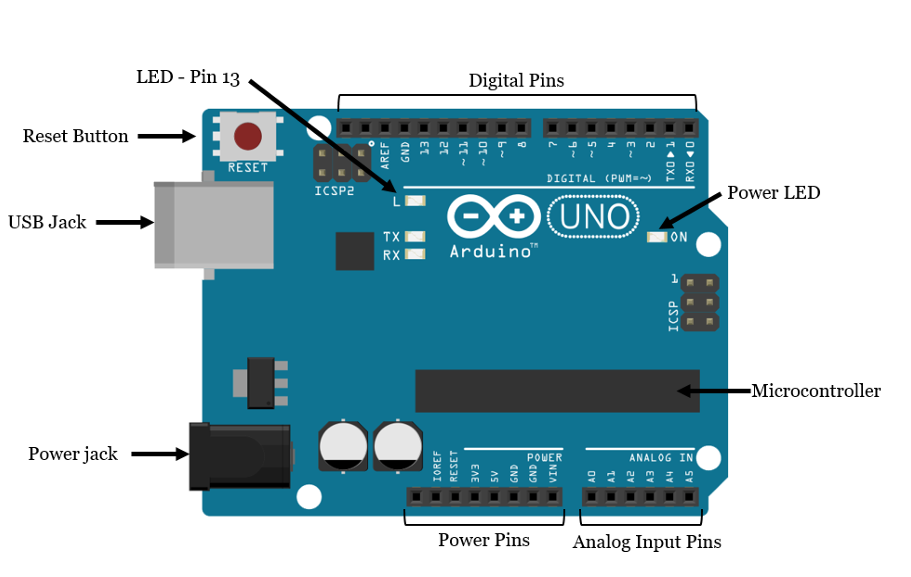
\includegraphics[width =0.8\textwidth]{ArduinoBoard.png}
            \end{center}
      
    
    Starting clockwise from the top center:
    \begin{itemize}
    \item Analog Reference pin (orange)
    \item Digital Ground (light green)
    \item Digital Pins 2-13 (green)
    \item Digital Pins 0-1/Serial In/Out - TX/RX (dark green
    \item  Reset Button - S1 (dark blue)
    \item  In-circuit Serial Programmer (blue-green)
    \item  Analog In Pins 0-5 (light blue)
    \item  Power and Ground Pins (power: orange, grounds: light orange)
    \item  External Power Supply In (9-12VDC) - X1 (pink)
    \item  Toggles External Power and USB Power (place jumper on two pins closest to desired supply) -
    SV1 (purple)
    \item  USB (used for uploading sketches to the board and for serial communication between the board
    and the computer; can be used to power the board) (yellow)
    \end{itemize}
    
    \par- These pins cannot be used for digital i/o (digitalRead and digitalWrite) if serial communication is also being used (e.g. Serial.begin).
        \subsubsection{Digital Pins}
        The digital pins on an Arduino board can be used for general purpose input and output via the pinMode(), digitalRead(), and digitalWrite() commands. Each pin has an internal pull-up resistor which
        can be turned on and off using digitalWrite() (w/ a value of HIGH or LOW, respectively) when the
        pin is configured as an input.
        \begin{itemize}
        \item Serial: 0 (RX) and 1 (TX). Used to receive (RX) and transmit (TX) TTL serial data.[1]
        \item External Interrupts: 2 and 3. These pins can be configured to trigger an interrupt on a low
        value, a rising or falling edge, or a change in value.
        \item PWM: 3, 5, 6, 9, 10, and 11. Provide 8-bit PWM output with the analogWrite() function. On
        boards with an ATmega8, PWM output is available only on pins 9, 10, and 11
        \end{itemize}
    
        \subsubsection{Analog Pins}
        The analog input pins support 10-bit analog-to-digital conversion (ADC) using the analogRead()
        function. Most of the analog inputs can also be used as digital pins: analog input 0 as digital pin 14
        through analog input 5 as digital pin 19.

        \subsubsection{Power Pins}
        \begin{itemize}
            \item \textbf{9V:} The input voltage to the Arduino board when it’s using an external power source (as opposed
            to 5 volts from the USB connection or other regulated power source). Different boards accept
            different input voltages ranges.
            \item \textbf{5V:} The regulated power supply used to power the microcontroller and other components on
            the board. This can come either from VIN via an on-board regulator, or be supplied by USB or
            another regulated 5V supply.
            \item \textbf{3.3V:} (Diecimila-only) A 3.3 volt supply generated by the on-board FTDI chip. 
                \item \textbf{GND:} Ground pins.
        \end{itemize}
        
        
    





    \pagebreak\section{Blinking \& Fading LED}

\subsection{Blinking LED}
LEDs are small, powerful lights that are used in many different applications. To start, we will work on blinking an LED, the Hello World of microcontrollers. It is as simple as turning a light on and off. Establishing this important baseline will give you a solid foundation as we work towards experiments that are more complex.

\subsubsection{Experiment URL}
     Use this \href{https://www.tinkercad.com/things/cJh2vPJHNMo?sharecode=pHXIFXpJnKTcQPuxdNKi-4YMURyigVNB9XbDgZYDrw8}{link} to get the \textbf{Tinkercad} simulation of this experiment.
    
\subsubsection{Objectives}
In this lesson, we will program the Arduino's GPIO output high level and low level (0V), and then make
the LED which is connected to the Arduino’s GPIO flicker with a certain frequency

\subsubsection{Necessary Components}
We will need the following components −
\begin{itemize}
    \item 1 x Breadboard
    \item 1 x Arduino Uno R3
    \item 1 x LED
    \item 1 x 330 $\Omega$ Resistor
    \item 2 × Jumper
\end{itemize}

\pagebreak\subsubsection{Circuit Diagram}
        \begin{figure}[!ht]
            \centering
            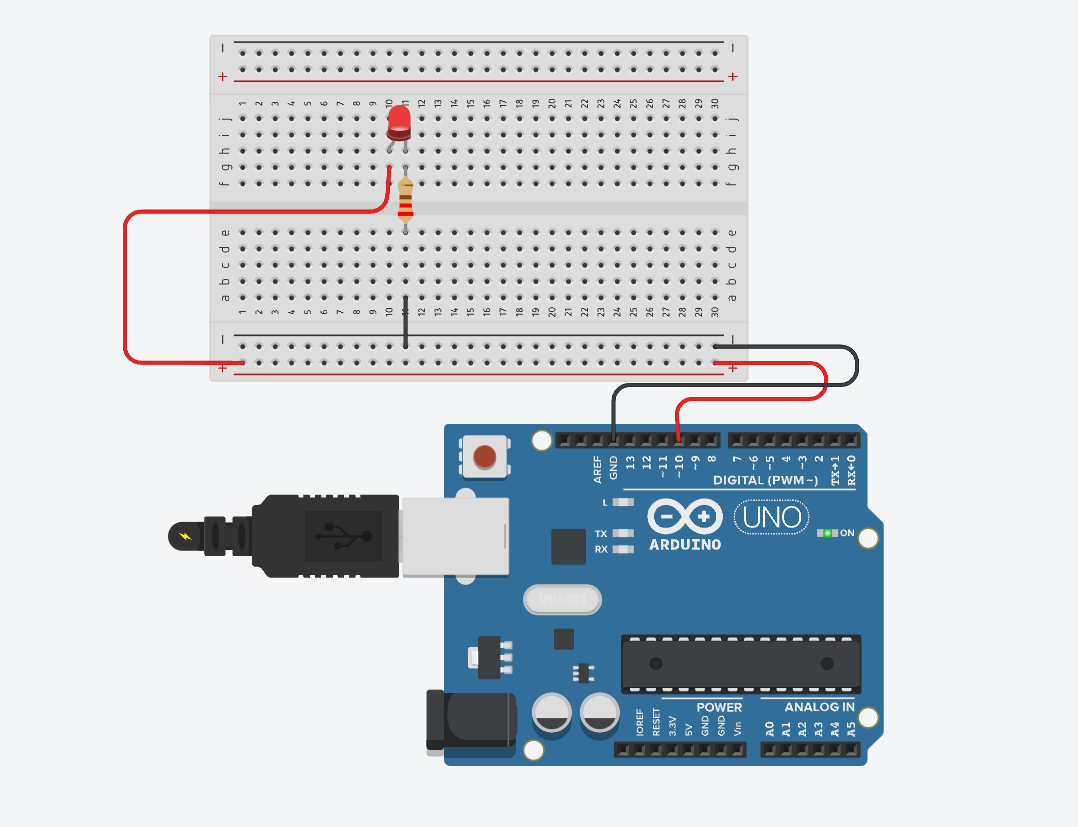
\includegraphics[width =0.75\textwidth]{images/BlinkingLED.png}
        %    \caption{Blinking LED circuit}
        \end{figure}
            
\subsubsection{Arduino Code}
    \begin{lstlisting}[style = Arduino]
    /* Blinking LED   */

int  ledPin = 10; //Initialize digital pin 10 set as LED output pin
int gap = 500; // Wait for 500 millisecond(s)

void setup()
{
  pinMode(ledPin, OUTPUT);
}

void loop()
{
  // turn the LED on (HIGH is the voltage level)
  digitalWrite(ledPin, HIGH);
  delay(gap); 
  // turn the LED off by making the voltage LOW
  digitalWrite(ledPin, LOW);
  delay(gap);
}
    \end{lstlisting}
 
\begin{comment}
\subsubsection{Conclusion}    
    We should see our LED turn on and off with the given delay. If the required output is not seen, we need to make sure we have assembled the circuit correctly, and have verified and uploaded the code to the board.
\end{comment}    
    
%%%%%%%%%%%%%%%%%%%%%%%%%%%%%%%%%%%%%%%%%%%%%%%%%%%%%%%%%%%%%%%%%%%%%%%%%%%%%%%%%%%%%%%%%%%%%%%%%%%%%%%%%%%%%%%%%%%%%%%%%%%
%%%%%%%%%%%%%%%%%%%%%%%%%%%%%%%%%%%%%%%%%%%%%%%%%%%%%%%%%%%%%%%%%%%%%%%%%%%%%%%%%%%%%%%%%%%%%%%%%%%%%%%%%%%%%%%%%%%%%%%%%%%

\pagebreak\subsection{Fading LED}

\subsubsection{Experiment URL}
Use this \href{https://www.tinkercad.com/things/dPLO4csum3h?sharecode=fTlXe0aOvAKUaa1xymJ71oC1m0_NHLRisRVjCh7YtyI}{link} to get the \textbf{Tinkercad} simulation of this experiment.
        
\subsubsection{Objectives}
This experiment demonstrates the use of the analogWrite() function in fading an LED off and on. AnalogWrite uses pulse width modulation (PWM), turning a digital pin on and off very quickly with different ratio between on and off, to create a fading effect.
\subsubsection{Necessary Components}
We will need the following components −
\begin{itemize}
    \item 1 x Breadboard
    \item 1 x Arduino Uno R3
    \item 1 x LED
    \item 1 x 330 $\Omega$ Resistor
    \item 2 × Jumper
\end{itemize}
\subsubsection{Schematic}
        \begin{figure}[!ht]
            \centering
            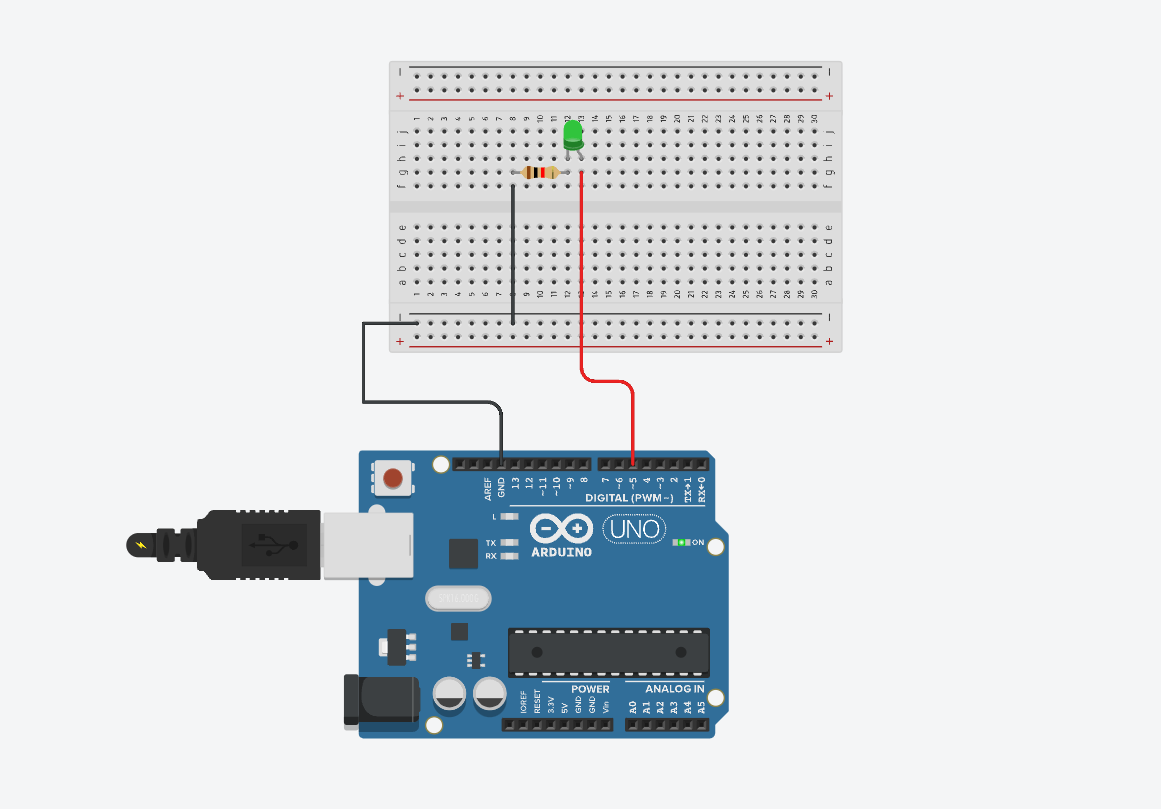
\includegraphics[width =0.75\textwidth]{images/FadingLED.png}
    %        \caption{Fading LED circuit}
        \end{figure}
            
\pagebreak\subsubsection{Arduino Code}
    \begin{lstlisting}[style = Arduino]
/*Fading LED*/

const int pinLED = 5; //declaring PWM pin 5 as LED output
int brightness = 0 ; //declaring LED initial condition
int fadeAmount = 5; // how many points to fade the LED by

void setup()
{
  pinMode(pinLED, OUTPUT); //initializing PWM pin 5 as LED output
  Serial.begin(9600);
}

void loop(){

  for (brightness = 0; brightness <= 255; brightness += fadeAmount){
  analogWrite(pinLED,brightness);
  delay(50); //interval for the brightenig effect
	}
	
  delay(500);  //wait for 500ms to run the loop again
  
  for (brightness = 255; brightness >= 0; brightness -= fadeAmount){
  analogWrite(pinLED,brightness);
  delay(50); //interval for the dimming effect
	}
  delay(500); //wait for 500ms to run the loop again
}\end{lstlisting}
    \pagebreak\section{Measurement of voltages (Below 5V and above)}
\subsection{Experiment URL}
    Use this \href{https://www.tinkercad.com/things/awpboVDdbxj?sharecode=uw7s84LgESyuaN5hnURGDUiU3aelHYsxpXATCcO_EfU}{link} to get the \textbf{Tinkercad} simulation of this experiment.
\subsection{Objectives}
We are going to make a simple digital voltmeter using the Arduino Uno R3, which can safely measure input dc voltages in 0 to 30V range. The Arduino board can be powered from a standard 9V battery pack or you can just use your desktop's USB port, as usual.

As you may well know, Arduino’s analog inputs can be used to measure DC voltage between 0 and 5V (when using the standard 5V analog reference voltage) and this range can be increased by using two resistors to create a voltage divider. The voltage divider decreases the voltage being measured to within the range of the Arduino analog inputs. Code in the Arduino sketch is then used to compute the actual voltage being measured.

\subsection{Necessary Components}
We will need the following components −
\begin{itemize}
\item 1 x Arduino Uno R3
\item 1 x Breadboard
\item 1 x 30V Power Supply
\item 1 x 1k$\Omega$ Resistor
\item 1 x 5k$\Omega$ Resistor
\item 1 x 16x2 LCD screen
\item 1 x USB A-B cable
\item Jumper Wires
\end{itemize}


\subsection{Circuit Diagram}
            \begin{center}
            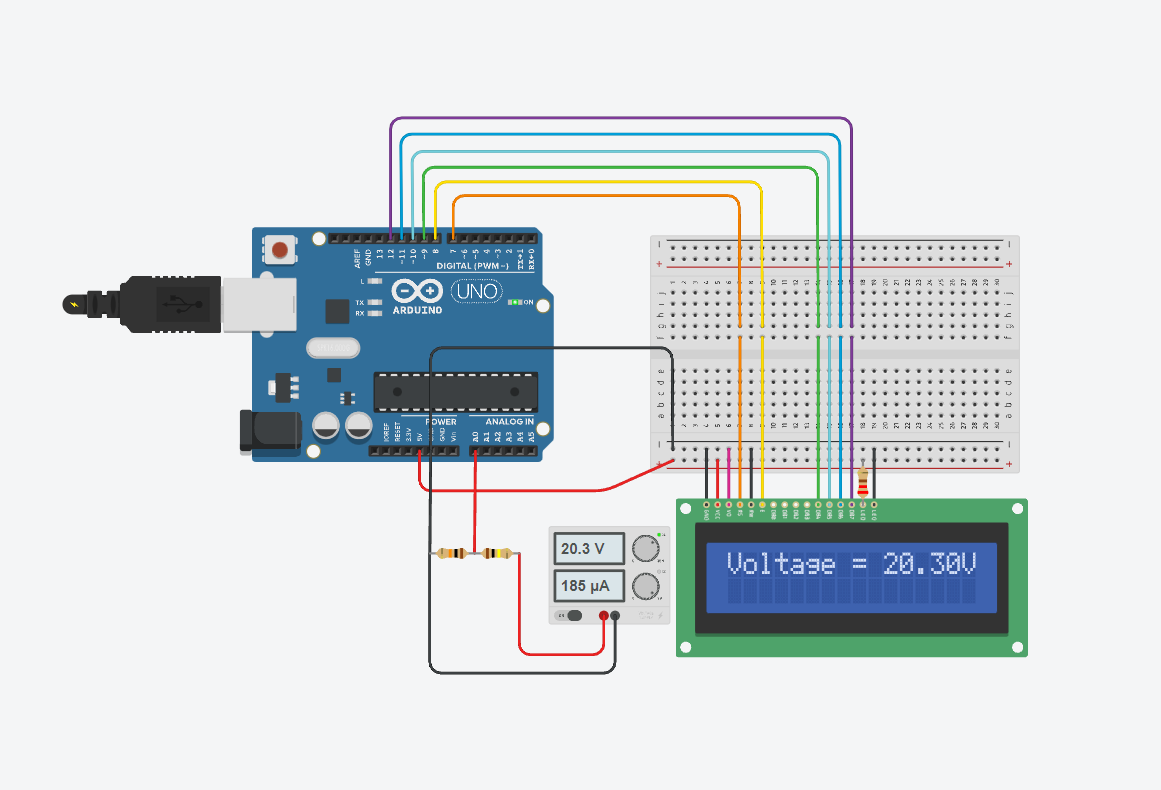
\includegraphics[width =0.85\textwidth]{images/measure_analog_voltage.png}
            \end{center}


\subsection{Formula for calculating voltage:}

\begin{equation}
    V_0 = (Val * 5.0) / 1023.00
\end{equation}
Here in these formula Val is the value that is read by Arduino as analog input, which is further multiplied by the voltage that is been supplied by Arduino and thus to get the Vout it is divided by the cycle of time that is covered after every bit to get the value.
\begin{equation}
    V_{in} = {V_{0}}~/~\frac{R2}{(R1+R2)}
\end{equation}
Using this formula we can convert the high voltages into the voltage range of Arduino (0 - 5V) using the voltage divider and measure any voltage using suitable resistor combinations. 

NOTE: Here there is no restriction on using the specified amount of resistors, one can vary it according to the availability of the resistors.


\pagebreak\subsection{Arduino Code}
    \begin{lstlisting}[style = Arduino]
/*Analog voltage measurement using Arduino*/

#include <LiquidCrystal.h>

//initialize the library by associating needed LCD interface pin
const int rs = 7, en = 8, d4 = 9, d5 = 10, d6 = 11, d7 = 12;

LiquidCrystal lcd(rs, en, d4, d5, d6, d7);

int analogIn = A0;
float v0 = 0.0;
float vin = 0.0;
float R1 = 5000.0; // resistance of R1 (5K) 
float R2 = 1000.0; // resistance of R2 (1K) 
int value;
void setup()
	{
   pinMode(analogIn, INPUT);
   lcd.begin(16, 2);
   lcd.setCursor(4,0);
   lcd.print("Voltmeter");
   delay(1000);
  	}

void loop()
	{
  value = analogRead(analogIn);  //read the value at analog input pin
  v0 = (value * 5.0) / 1023.0; // voltage value as read by A0
  vin = v0 / (R2/(R1+R2)); // voltage reverted back to original

  lcd.clear();
  lcd.setCursor(0, 0);
  lcd.print("Voltage = ");
  lcd.print(vin);
  lcd.print("V");
  delay(100);
}
    \end{lstlisting}    
    \pagebreak\section{Interfacing a seven segment display}
\subsection{Experiment URL}
    Use this \href{https://www.tinkercad.com/things/cBjJt1Np6D3?sharecode=MGQeyKRCp2DAykyyOVjQAholeCilkMIFth6zI349h3c}{link} to get the \textbf{Tinkercad} simulation of this experiment.
    
\subsection{Objectives}


\subsection{Necessary Components}
We will need the following components −
\begin{itemize}
\item 1 x seven segment display (common cathode)
\item 1 x Arduino UNO R3
\item 1 x breadboard
\item 1 x 1k$\Omega$ resistors (1/4 W)
\item jumper wires
\end{itemize}
\subsection{Circuit Diagram}
        \begin{figure}[!h]
            \centering
            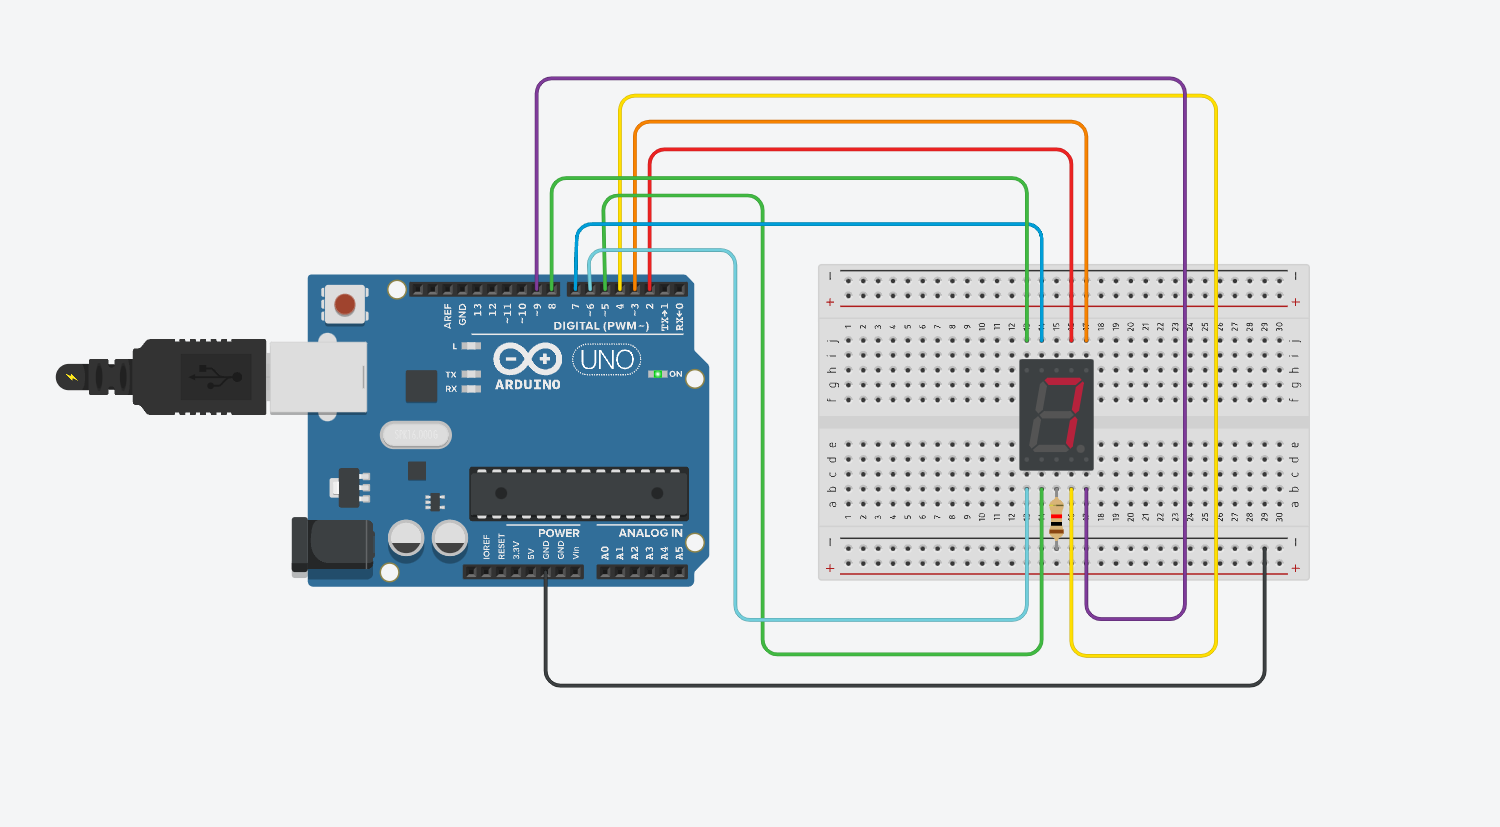
\includegraphics[width =0.85\textwidth]{images/seven_segment_display.png}
            \caption{Interfacing seven segment display with Arduino}
        \end{figure}

\pagebreak\subsection{Arduino Code}
    \begin{lstlisting}[style = Arduino]
/*Interfacing a seven segment display using Arduino*/
int i;
int pinA = 2;
int pinB = 3;
int pinC = 4;
int pinD = 5;
int pinE = 6;
int pinF = 7;
int pinG = 8;
int pinDP = 9;

void setup()
{
  for ( i = 2; i <= 9; i++){
  pinMode(i, OUTPUT);
}
}

void loop()
{
  // display 0
  digitalWrite(2, HIGH);
  digitalWrite(3, HIGH);
  digitalWrite(4, HIGH);
  digitalWrite(5, HIGH);
  digitalWrite(6, HIGH);
  digitalWrite(7, HIGH);
  digitalWrite(8, LOW);
  digitalWrite(9, LOW);
  delay(1000); // Wait for 1000 millisecond(s)
  // display 1
  digitalWrite(2, LOW);
  digitalWrite(3, HIGH);
  digitalWrite(4, HIGH);
  digitalWrite(5, LOW);
  digitalWrite(6, LOW);
  digitalWrite(7, LOW);
  digitalWrite(8, LOW);
  digitalWrite(9, LOW);
  delay(1000); // Wait for 1000 millisecond(s)
  // display 2
  digitalWrite(2, HIGH);
  digitalWrite(3, HIGH);
  digitalWrite(4, LOW);
  digitalWrite(5, HIGH);
  digitalWrite(6, HIGH);
  digitalWrite(7, LOW);
  digitalWrite(8, HIGH);
  digitalWrite(9, LOW);
  delay(1000); // Wait for 1000 millisecond(s)
  // display 3
  digitalWrite(2, HIGH);
  digitalWrite(3, HIGH);
  digitalWrite(4, HIGH);
  digitalWrite(5, HIGH);
  digitalWrite(6, LOW);
  digitalWrite(7, LOW);
  digitalWrite(8, HIGH);
  digitalWrite(9, LOW);
  delay(1000); // Wait for 1000 millisecond(s)
  // display 4
  digitalWrite(2, LOW);
  digitalWrite(3, HIGH);
  digitalWrite(4, HIGH);
  digitalWrite(5, LOW);
  digitalWrite(6, LOW);
  digitalWrite(7, HIGH);
  digitalWrite(8, HIGH);
  digitalWrite(9, LOW);
  delay(1000); // Wait for 1000 millisecond(s)
  // display 5
  digitalWrite(2, HIGH);
  digitalWrite(3, LOW);
  digitalWrite(4, HIGH);
  digitalWrite(5, HIGH);
  digitalWrite(6, LOW);
  digitalWrite(7, HIGH);
  digitalWrite(8, HIGH);
  digitalWrite(9, LOW);
  delay(1000); // Wait for 1000 millisecond(s)
  // display 6
  digitalWrite(2, HIGH);
  digitalWrite(3, LOW);
  digitalWrite(4, HIGH);
  digitalWrite(5, HIGH);
  digitalWrite(6, HIGH);
  digitalWrite(7, HIGH);
  digitalWrite(8, HIGH);
  digitalWrite(9, LOW);
  delay(1000); // Wait for 1000 millisecond(s)
  // display 7
  digitalWrite(2, HIGH);
  digitalWrite(3, HIGH);
  digitalWrite(4, HIGH);
  digitalWrite(5, LOW);
  digitalWrite(6, LOW);
  digitalWrite(7, LOW);
  digitalWrite(8, LOW);
  digitalWrite(9, LOW);
  delay(1000); // Wait for 1000 millisecond(s)
  // display 8
  digitalWrite(2, HIGH);
  digitalWrite(3, HIGH);
  digitalWrite(4, HIGH);
  digitalWrite(5, HIGH);
  digitalWrite(6, HIGH);
  digitalWrite(7, HIGH);
  digitalWrite(8, HIGH);
  digitalWrite(9, LOW);
  delay(1000); // Wait for 1000 millisecond(s)
  // display 9
  digitalWrite(2, HIGH);
  digitalWrite(3, HIGH);
  digitalWrite(4, HIGH);
  digitalWrite(5, LOW);
  digitalWrite(6, LOW);
  digitalWrite(7, HIGH);
  digitalWrite(8, HIGH);
  digitalWrite(9, LOW);
  delay(1000); // Wait for 1000 millisecond(s)
}

\end{lstlisting} 
    \pagebreak\section{DHT22 Temperature and Humidity Sensor}
\subsection{Experiment URL}
    Use this \href{https://wokwi.com/projects/333082438824624723}{link} to get the \textbf{Wokwi} simulation of this experiment.
    
\subsection{Objectives}
DHT22 is a Humidity and Temperature Sensor, which generates calibrated digital output. DHT22 can be interface with any microcontroller like Arduino, Raspberry Pi, etc. and get instantaneous results. DHT22 is a low cost humidity and temperature sensor which provides high reliability and long term stability.
In this project, we will build a small circuit to interface Arduino with DHT22 Temperature and Humidity Sensor. One of the main applications of connecting DTH22 sensor with Arduino is weather monitoring.

\subsection{Necessary Components}
We will need the following components −
\begin{itemize}
\item 1 x Arduino Uno R3
\item 1 x Breadboard
\item 1 x DHT22 temperature and humidity sensor
\item 1 x 10k $\Omega$ potentiometer
\item 1 x 16x2 LCD screen
\item 1 x USB A-B cable
\item Jumper Wires
\end{itemize}

\subsection{Circuit Diagram}
            \begin{center}
            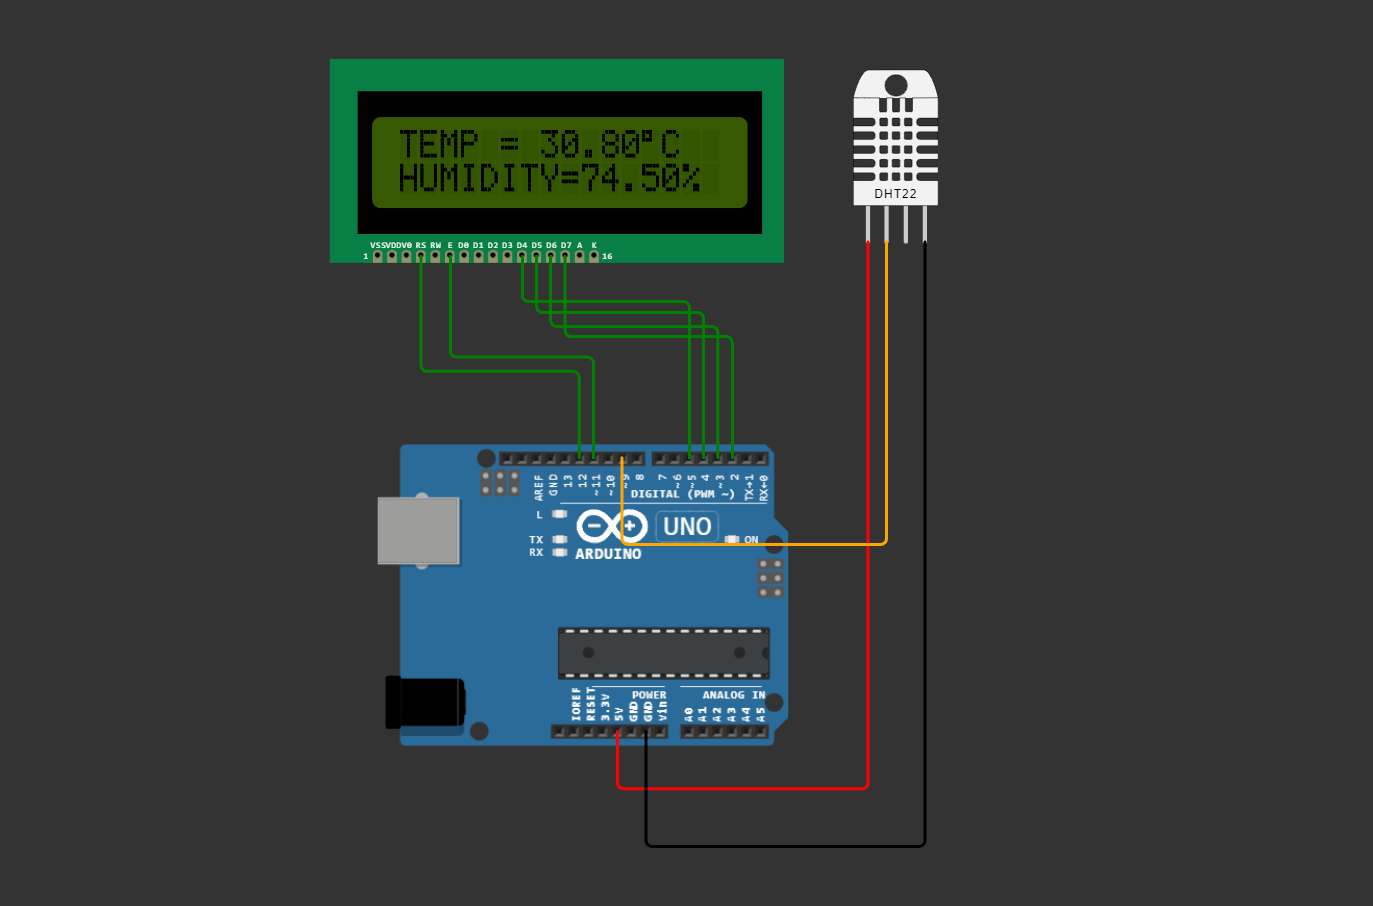
\includegraphics[width =0.7\textwidth]{images/dht22Circuit.png}
            \end{center}

\subsection{Arduino Code}
    \begin{lstlisting}[style = Arduino]
#include <LiquidCrystal.h>
#include <DHT.h>

#define DHTPIN  9
#define DHTTYPE DHT22 


LiquidCrystal lcd(12, 11, 5, 4, 3, 2); // initialize the library with the numbers of the interface pins
DHT dht(DHTPIN, DHTTYPE); //initialize DHT sensor pin


void setup() {
  dht.begin();
  lcd.begin(16, 2); // set up the LCD's number of columns and rows
  
  lcd.setCursor(0,0);

  lcd.print("Initializing....");
  delay(1000);

}

void loop() {
  float temp = dht.readTemperature();
//float tempF = dht.readTemperature(true);
  float hum = dht.readHumidity();

  lcd.clear();
  
  lcd.setCursor(0,1);
  lcd.print("HUMIDITY=");
  lcd.print(hum);            //Displaying humidity
  lcd.print("%");

  lcd.setCursor(0,0);
  lcd.print("TEMP = ");
  lcd.print(temp);            //Displaying temperature in C
  lcd.print((char)223);
  lcd.print("C");
  delay(2000);
}
 
 \end{lstlisting} 
    \pagebreak\section{Data logger for studying charging and discharging of RC circuit}

\subsection{Experiment URL}
    Use this \href{https://www.tinkercad.com/things/awg0vQADVPP?sharecode=lBK08ktzr9HdJWinGq0Pj3PSK_MzsvQ5bzUg1wqTPac}{link} to get the \textbf{Tinkercad} simulation of this experiment.
    
\subsection{Objectives}
If a capacitor of capacitance C (in farads), initially charged to a potential $V_0$ (volts) is connected across a resistor R (in ohms), a time-dependent current will flow according to Ohm’s law. This situation is shown by the RC (resistor-capacitor) circuit below when the switch is closed.  As the current flows, the charge q is depleted, reducing the potential across the capacitor, which in turn reduces the current. This process creates an exponentially increasing voltage, modeled by
    \begin{equation}
        V_C(t)=V_0(1−e^{-\frac{t}{R.C}})
    \end{equation} 
The rate of the decrease is determined by the product RC, known as the time constant of the circuit. A large time constant means that the capacitor will discharge slowly.  The same time constant RC describes the rate of charging as well as the rate of discharging. The graph shows how the voltage across the capacitor $V_C$ and the voltage across the resistor $V_R$ vary with time when charging. The relationships are found by integrating the expression for the voltage on a capacitor. The voltage over the resistor while charging is given by:                                  
    \begin{equation}
        V_R(t)=V_0(e^{-\frac{t}{R.C}})
    \end{equation} 

We will be using a square wave voltage supply to provide the ‘switching’ between open and closed for our RC circuit. We will then examine the plots in LoggerPro of the voltages over both the capacitor and the resistor for the charging and discharging of the RC circuit. We will compare the curve fits to the theoretical predictions for the voltage and the time constant for the circuit.

The main objective of this Arduino investigation of the RC circuit is the experimental verification of the formulas for the time-varying voltage and electric current for the charging or discharging capacitor. A secondary objective is to provide an alternative to more expensive commercial laboratory materials and, at the same time, to expose the students to the underlying electronics and computer programming that would have otherwise been hidden from sight.

\subsection{Necessary Components}
We will need the following components −
\begin{itemize}
\item 1 x Arduino Uno R3
\item 1 x Breadboard
\item 1 x 100 $\mu$F capacitor
\item 1 x 10k $\Omega$ resistor
\item 1 x USB A-B cable
\item Jumper Wires
\end{itemize}

\subsection{Circuit Diagram}
            \begin{center}
            \includegraphics[width =0.85\textwidth]{images/RC_charging_discharging_circuit.png}
            \end{center}


\subsection{Arduino Code}

\begin{lstlisting}[style = Arduino]
/*DataLogger for charging and discharging of the RC Circuit */
int chargePin = 8;
int capPin = A5;

const float C = 100.0; //capacitance in uF
const float R = 10.0; //capacitance in kOhms
const float timeConstant = (R*C)/1000;

float startTimeCharge;
float startTimeDischarge;
float elapsedTimeCharge;
float elapsedTimeDischarge;
float rawInput;
float voltage;
float percentCharge;

void setup() {
  Serial.begin(9600); 
  Serial.print("The time constant of the RC circuit is: ");
  Serial.print(timeConstant);
  Serial.println("s");
  
  pinMode(chargePin, OUTPUT);
  digitalWrite(chargePin, LOW);
}

void loop() {
  rawInput = analogRead(capPin);
  voltage = (rawInput/1024.0)*5; 
  
  /////////Charging/////////////
  
  digitalWrite(chargePin, HIGH); 
  startTimeCharge = millis(); //
    
  
  while (rawInput < 1023.0) {
  rawInput = analogRead(capPin);
  voltage = (rawInput/1024.0)*5;
  float elapsedTimeCharge = (millis() - startTimeCharge) / 1000.0;  //  
  Serial.print(voltage, 3); // voltage in Volts 
  Serial.print("\t");
  Serial.print(elapsedTimeCharge, 3); //time in seconds 
  Serial.print("\n");
  delay(100);   
  }
  
 /////////Discharging/////////////
  
  digitalWrite(chargePin, LOW); 
  startTimeDischarge = millis(); //
  
  
  while (rawInput > 0.0) {   
  rawInput = analogRead(capPin);
  voltage = (rawInput/1023.0)*5;
  float elapsedTimeDischarge = (millis() - startTimeDischarge) / 1000.0;    
  Serial.print(voltage, 3); // voltage in Volts 
  Serial.print("\t");
  Serial.print(elapsedTimeDischarge, 3); //time in seconds 
  Serial.print("\n");
  delay(100);   
  }
}
\end{lstlisting}

\subsection{Charging and discharging plot}
        \begin{figure}[!ht]
            \centering
            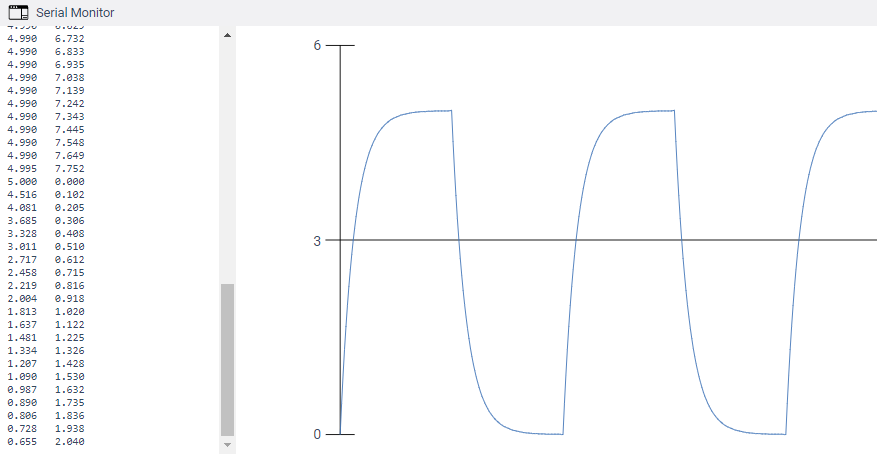
\includegraphics[width =0.85\textwidth]{images/rc_realtime_plot.png}
            \caption{Data logging real time charging and discharging}
        \end{figure}
We copied and pasted the two columns (voltage and time) of the serial monitor in a text file and plotted the data using \textbf{Python}'s plotting library \textbf{Matplotlib}.

\vspace{10pt} \begin{lstlisting}[language = Python]
import matplotlib.pyplot as plt
import numpy as np

voltage = []
time = []

#X, Y = np.loadtxt("capacitor_charging.txt", delimiter=',', unpack=True)
f = open("capacitor_discharging.txt","r")
i = []

for i in f:
    i = i.replace('\n', ' ')
    i = i.replace('\t', ' ')
    i = i.split()
    voltage.append(float(i[0]))
    time.append(float(i[1]))
print(voltage)
print(time)
plt.plot(time, voltage, "--", label = "voltage vs time")
plt.title('Capacitor Disharging')
plt.xlabel('Time (s)')
plt.ylabel('Voltage (V)')
plt.legend()
plt.show()
\end{lstlisting}

        \begin{wrapfigure}{c}{\textwidth}
            \centering
            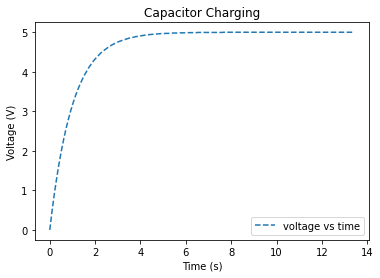
\includegraphics[scale=0.5]{images/rc_charging_plot.png}
            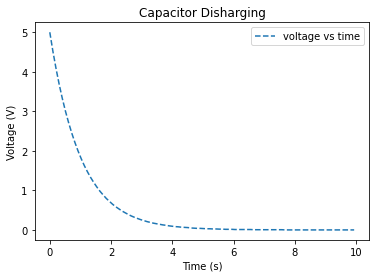
\includegraphics[scale=0.5]{images/rc_discharging_plot.png}
            \caption{RC Charging and discharging plot}
        \end{wrapfigure}

 
    
%---------------------------------------------------------------------------------------------------------


\end{document}